\chapter{论文组织结构与时间安排}

\section{论文组织结构}

第一章为绪论,主要介绍介观尺度的地理现象,以及空间交互如何对其产生影响。本文利用高精度的交互数据和理论模型,解释了产业分化及其在空间上的固化(fixation)过程、交互模式的稳定性、以及如何从数据中提取出关键的观测维度。

第二章是利用扩散映射法提取高维地理数据的关键信息。本章首先展示扩散映射法的理论基础,近期其在城市研究中的研究进展,以及面临的问题:无法针对问题进行定制结果,以及对重复的统计量不够鲁棒。其次,我们将描述我们对上述问题的解决方案:引入多维相似性指标,进行介观降维;以及引进负相似性来描述城市空间中的相斥结构的形成机制。最后,我们将通过对英美两国的人口普查数据的改进扩散映射结果,来展示城市中一些对偶结构、特定尺度空间组织的模式发现。

第三章是城市内交互系统的稳定性分析。本章分析了城市面对外来冲击时,居民受影响程度的扩散状况。首先我们根据城市元人口交互矩阵和冲击向量构建了交互的扩散矩阵,并由此定义城市交互稳定性。进而,我们寻找交互系统的一些守恒量和稳定性的确定条件。最后,利用美国15个主要城市2020年的人类移动性数据量化新冠病毒肺炎在各个城市内部传播的稳定性时序变化。通过研究试图进一步发现控制介观尺度上空间交互对于控制疫情的有效性,以及当发病率高到一定程度时控制介观结构之间的交互是否已经于事无补,是否严格的居家令才能使疫情得到控制。

第四章是从众心理驱动下的介观模式形成。我们通过考察三元关系传播意愿-二元关系传播疾病的模型,反映了心理因素对二元关系的影响。我们通过主方程的方法构建一个患病比例和戴口罩比例共同演化的非线性系统。并通过对其$(0,0)$, $(1,0)$, $(0,1)$, $(1,1)$附近稳定性的讨论,得到了一个达成“社会共识”的充要条件。最后,我们在多种真实网络上验证我们的结果,得到较为一般的性质。

第五章为结论。我们以介观尺度为切入点,探究了交互模式的形成、稳定性,以及如何从数据中提取不同主题交互的模式。结合研究中的不足,为进一步研究提出展望。

\section{研究内容框架、技术方法与可行性}

研究内容框架如图~\ref{fig:frame}所示。

\begin{figure}[h]
    \centering
    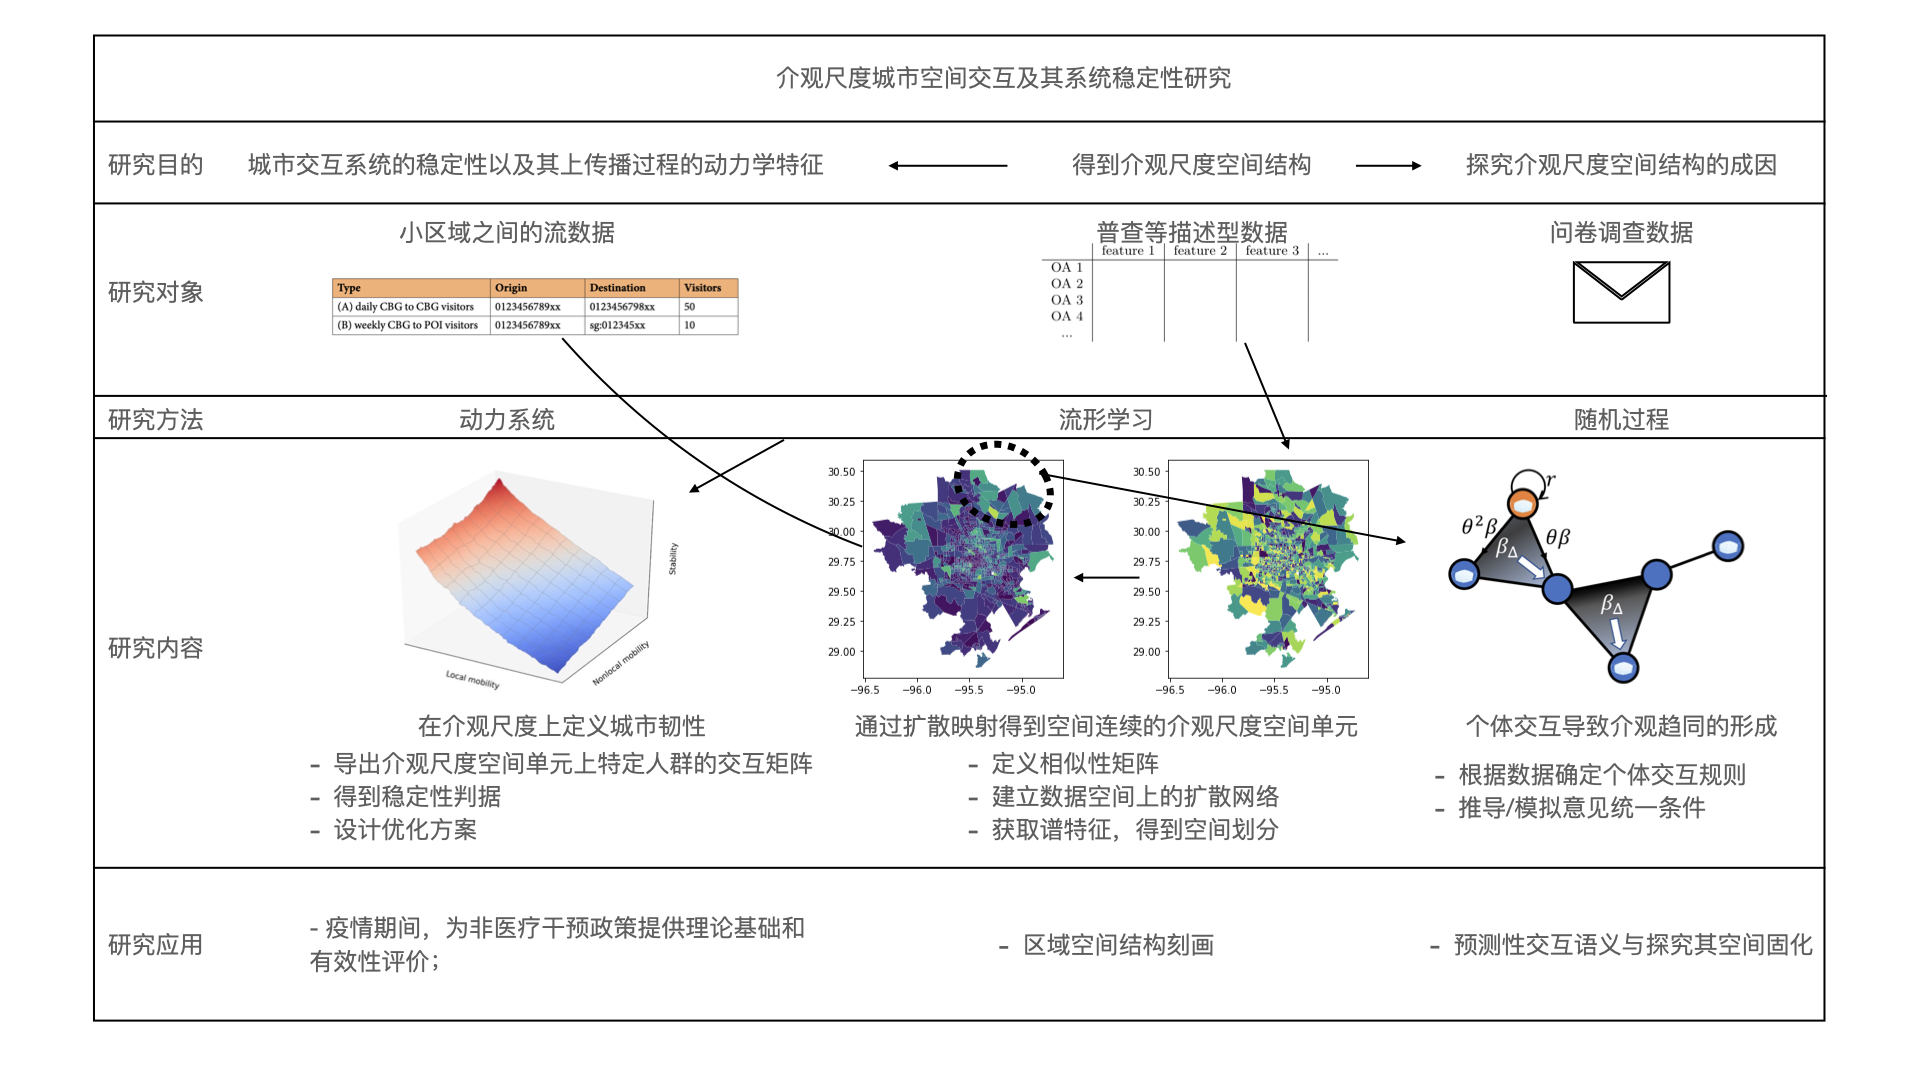
\includegraphics[width = 0.99\linewidth]{Figs/开题流程图.jpeg}
    \caption{论文研究内容与框架。本文先将研究尺度确定为可以最大反映城市动态确定性的介观尺度。以此为纲,向更大的尺度探究城市中传播过程的稳定性问题;向更小的尺度研究介观尺度空间模式的形成规律。}
    \label{fig:frame}
\end{figure}

% 可行性:数据条件、方法应用能力、实验室计算条件等
本文所提出的研究有很高的可行性。数据方面,笔者已通过官方网站获取了开源的我国、英国、以及美国的人口普查数据以支撑介观尺度空间单元提取的工作;引用\cite{kang2020multiscale}中提供的美国的2020年全国尺度的人类移动性数据和县一级的病例时间序列以支撑传播过程稳定性的工作;小范围的问卷调查数据以支撑介观尺度模式形成的工作。方法应用能力方面,本文涉及的三个工作都有较为完善的理论基础和实用能力,受随机性影响比较小,为政策制定空间范围、疫情防控尺度确定、以及面向公众宣传力度的决策都有着直观而鲁棒的应用前景。计算条件方面,Geosoft实验室拥有多台高性能服务器,亦申请了未名超算服务器来支持我们的工作。总之,本文涉及工作的实验条件十分完备。

\section{时间进度安排}

2021 年 7 月,完成局部交互模式形成和交互稳定性的小论文投稿;

2021 年 11 月,整理相关领域研究工作及最新进展,归纳总结现存研究问题,根据开题报告答辩情况完善研究框架;

2021 年 12 月至 2022 年 6 月,根据研究计划进行具体的工作,整理实验结果,完成博士论文初稿;

2022 年 10 月,结合导师意见完善博士论文;

2023 年 4 月,完成博士论文,开展博士论文答辩工作;

2023 年 5 月至 2023 年 6 月,参照评审意见对博士论文进行修改,并完成学位论文提交。